\section{Domain Concepts}
\label{sec:domain-concepts}
Before discussing the requirements, in order to get a better grasp of the project, based on its decomposition, the following concepts and terms are believed to be important and relevant:
\begin{itemize}
    \item Admin user – A type of user that has a better understanding of the navigation system and application and will be responsible for managing and measuring data.
    \item Application Programming Interface (API) – a set of methods used to communicate between software components.
    \item REpresentational State Transfer (REST) – a style of architecture that defines properties based on HTTP requests. The operations available through HTTP requests are GET, POST, PUT, PATCH and DELETE.
        \begin{itemize}
            \item GET request to /resources – Will retrieve all the resources.
            \item POST request to /resources – Will add a new resource.
            \item PUT request to /resources/:resource – Will add or overwrite the resource.
            \item PATCH request to /resources/:resource – Will partially update the resource specified.
            \item DELETE request to /services/:service – Will delete the specified service. If a service is not included, the operation will delete all the services.
        \end{itemize}
    \item CRUD – is an acronym for create, read, update and delete, which are the basic operations of a database.
    \item Raspberry Pi – A small single-board computer.
\end{itemize}
\newpage

\section{System Components}
In order to fully understand the functional requirements that are going to be defined in section \ref{sec:requirements}, it is very important to visualise the organisation of the system. This can be done by using figure \ref{fig:high-level-organisation}. The components have been separated into the presentation layer, which displays the services available by communicating with the lower layers, the logic tier, where controls the system's main functionalities, and the data tier, which houses the database servers (the data is kept independent of the other layers) \cite{three-tier}.

\begin{figure}[H]
    \centering
    \fbox{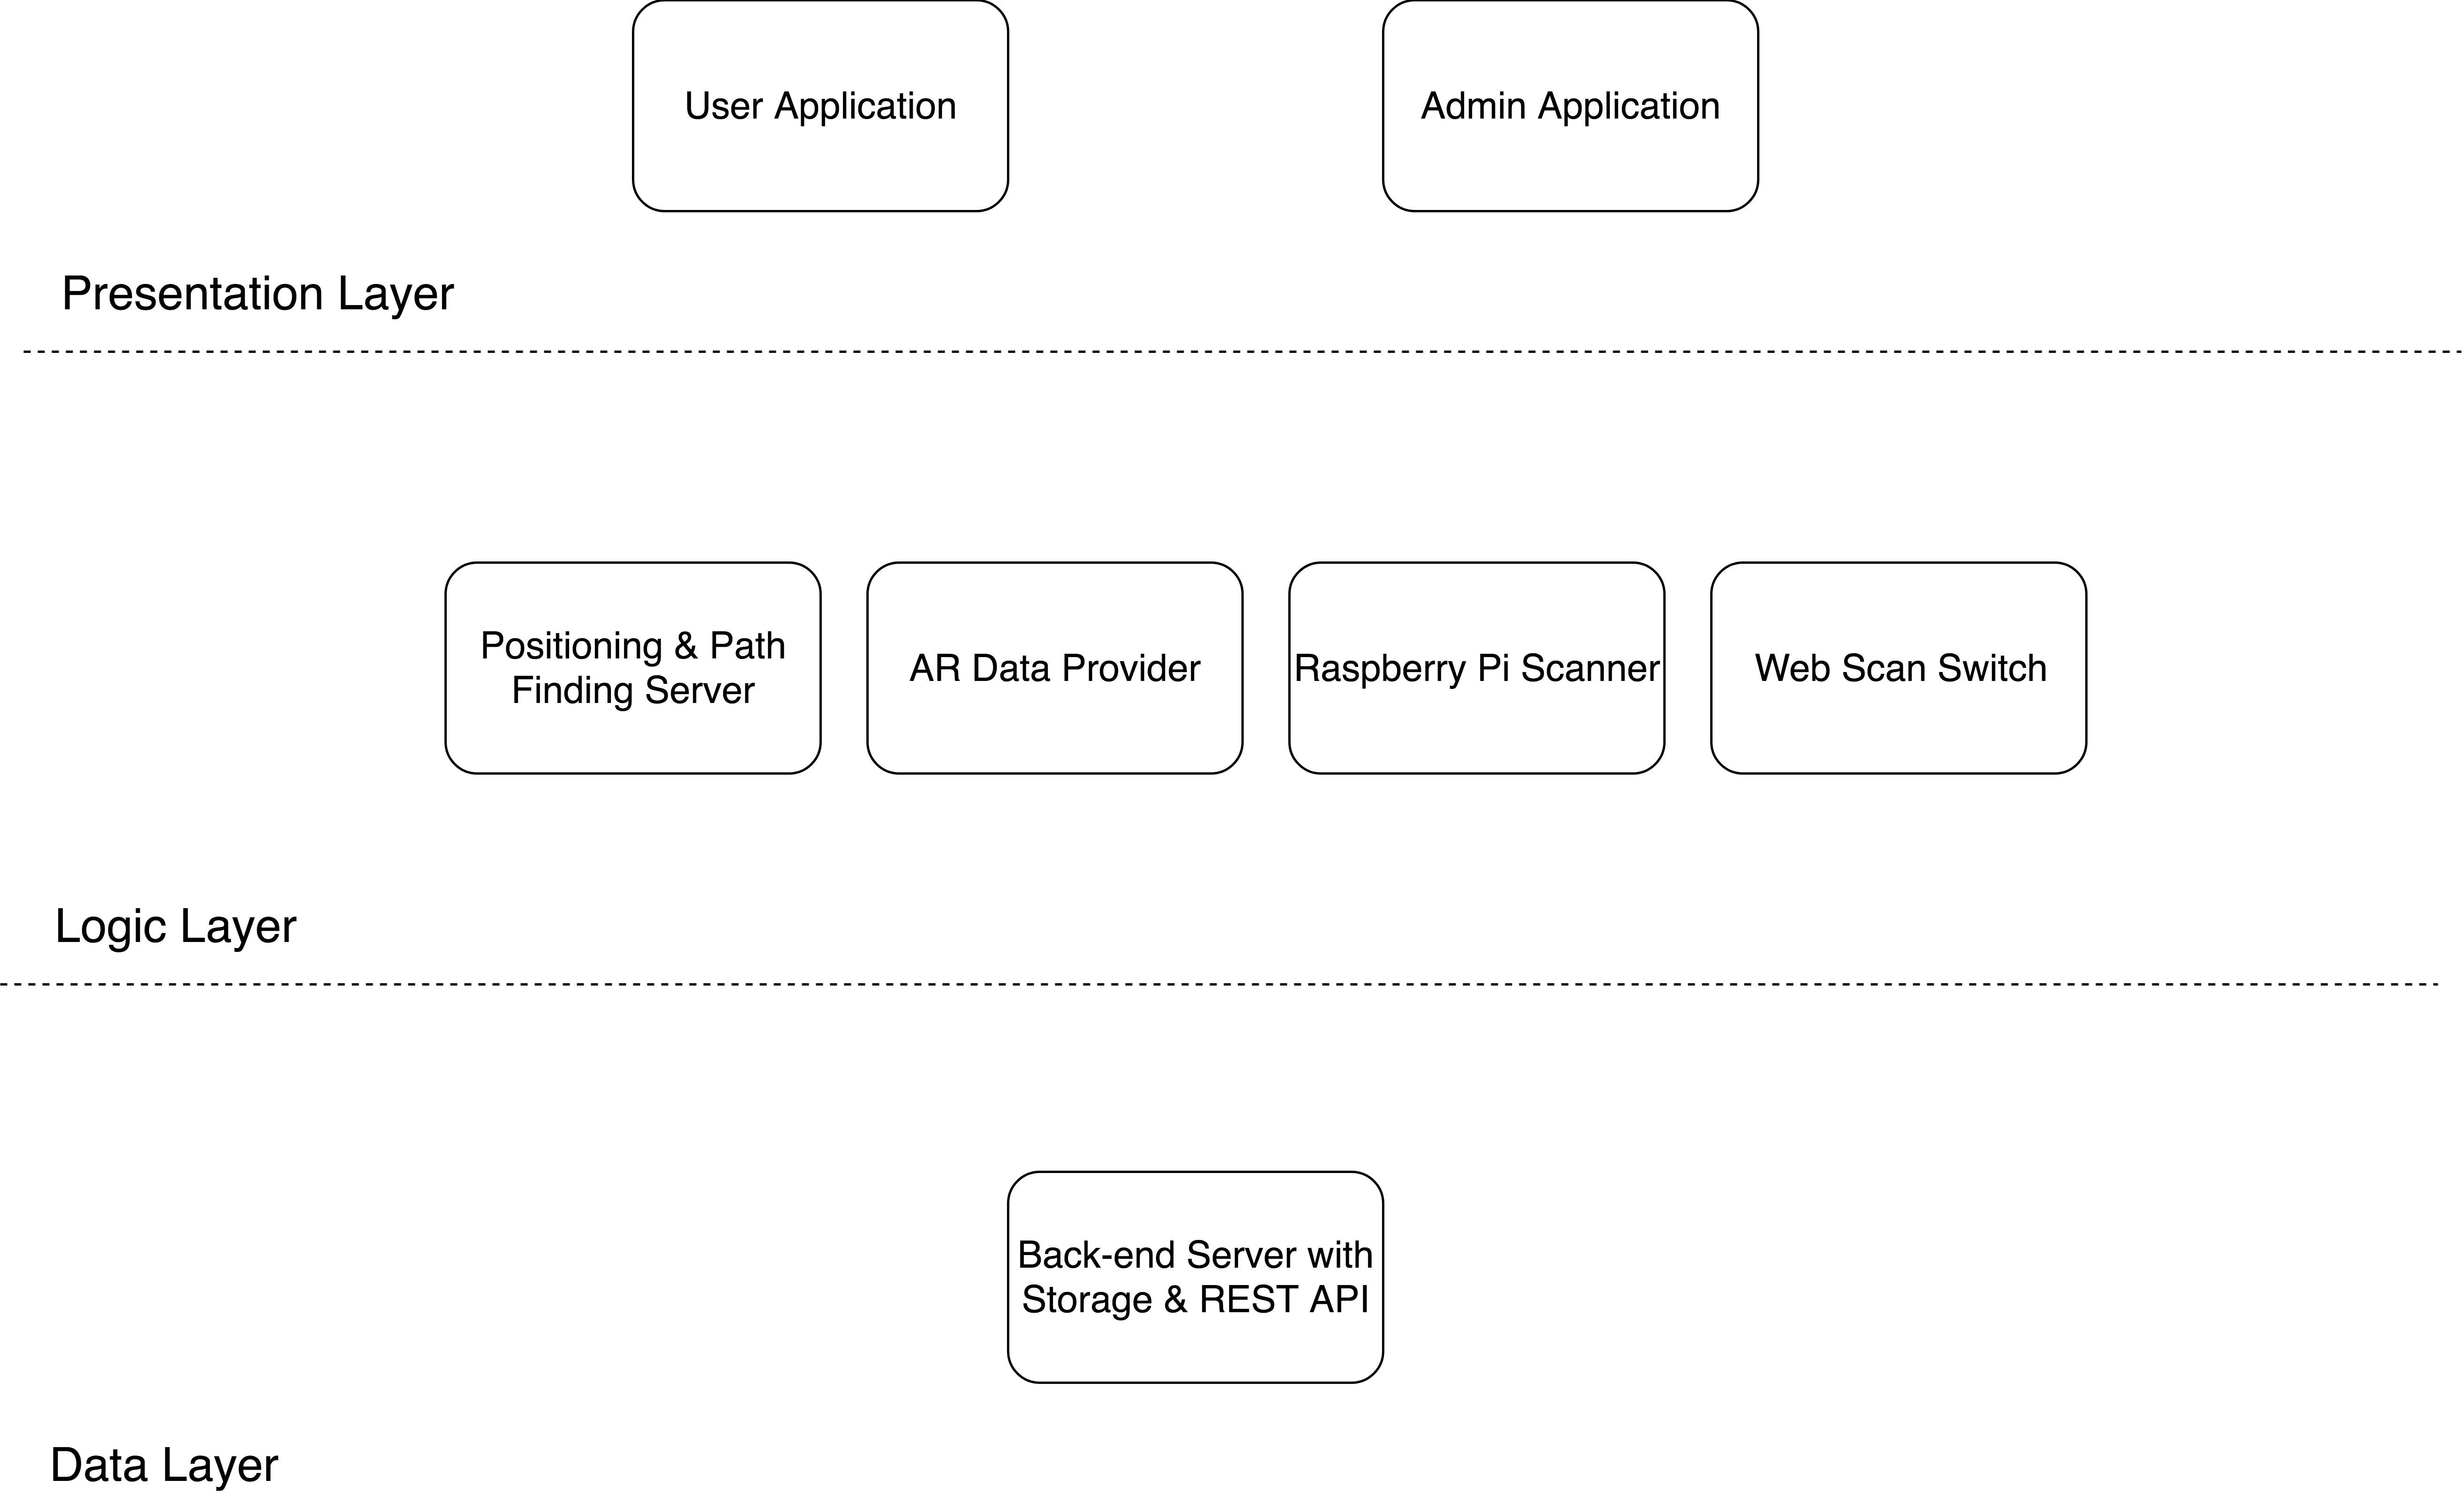
\includegraphics[width=350px, height=213px]{RequirementsSpecification/high-level-diagram.png}}
    \caption{High Level Organisation of the System. The round rectangles represent the components for which the requirements are defined in this chapter. These components have been organised in layers, using the tasks that they are performing.}
    \label{fig:high-level-organisation}
\end{figure}

\newpage
\section{Functional Requirements}
\label{sec:requirements}
The requirements have been divided for each component that has been developed. These components are: an admin iOS mobile application, a user iOS mobile application, a back-end server that manages the storage through a RESTful API, a back-end server to manage positioning and navigation, and a data provider for AR. Finally, a Raspberry Pi will be used to scan and upload Wi-Fi measurements, due to the limitation imposed on iOS, which will be detailed in the Conclusion chapter. The connection between the the mobile device and Raspberry Pi will be made through another web application which will act as a on-off switch that will let the Raspberry Pi know when it is time to scan.

The specific requirements for each component are detailed:

\subsection{Admin Mobile Application Requirements}
\label{sec:admin-requirements}
\begin{itemize}
    \item AM1 – Admin should add a room by providing a name for it. 
    \item AM2 – In the list of rooms, the admin user should be able to delete a room along with the data in it.
    \item AM3 – Admin should be able to select a room and start measuring Wi-Fi data for that room.
    \item AM4 – Admin should be able to reset the data measured so far for a specific room.
\end{itemize}

\subsection{User Mobile Application Requirements}
\label{sec:user-mobilde-requirements}
\begin{itemize}
    \item UM1 – User should be able to see their current location.
    \item UM2 – User should be able to see a list of registered rooms.
    \item UM3 – User should be able to search for a destination (a room).
    \item UM4 – User should receive instructions on how to get to the selected destination.
    \item UM5 – User should be able to receive an estimated arrival time from the starting position to the destination.
    \item UM6 – User should be able to use their mobile phone's camera to see directions towards the selected destination.
    \item UM7 – User should be able to see information about the timetable of a room.
    \item UM8 – User should be able to see information about the availability of computers in a room.
\end{itemize}

\subsection{Back-end Server with storage and REST API Requirements}
\label{sec:server-api}
\begin{itemize}
    \item BAPI1 – Database should store, update and delete rooms.
    \item BAPI2 – Back-end should store relevant data about rooms, such as Wi-Fi strengths positions.
    \item BAPI3 – The REST API should provide a link to get data from the database.
    \item BAPI4 – the REST API should provide a link to upload and update data in the database.
\end{itemize}

\subsection{Positioning \& Path Finding Server Requirements}
\label{sec:navigation-server}
\begin{itemize}
    \item PPF1 – The server should be able to determine the current location of the user.
    \item PPF2 – The server should be able to create a route and calculate the route's distance, given a starting position and destination.
\end{itemize}

\subsection{AR Data Provider}
\label{sec:ar-data-provider}
\begin{itemize}
    \item ARDP1 – The provider should supply the mobile application with an image of the timetable for the room that data has been requested for.
    \item ARDP2 – The provider should supply the mobile application with a status text of the availability of the computers in the room data has been requested for.
\end{itemize}

\subsection{Raspberry Pi Scanner Requirements}
\label{sec:rasp-pi-scanner}
\begin{itemize}
    \item RPS1 – Scan Wi-Fi networks around and store the signal strength, the MAC address and the network name locally.
    \item RPS2 – Upload the data measured in the database when requested, using the API from 3.2.3.
    \item RPS3 – Check continuously if data is needed every 2 seconds.
\end{itemize}

\subsection{Web Scan Switch Requirements}
\label{sec:web-scan-switch}
\begin{itemize}
    \item WSS1 – Have a Boolean flag to know if data needs to be scanned or not.
    \item WSS2 – The component should be able to temporarily store some measurement data. This data is going to be used to compare to already measured data in the process of positioning a user.
\end{itemize}

\section{Non-functional Requirements}
\begin{itemize}
    \item Extensibility – The system should have an implementation that can easily grow in features and capabilities at any given moment. These features should be added whilst minimising the impact to the existing system functions
    \item Interoperability – The subsystems should be able to fully integrate with other subsystems in order to provide maximum flexibility.
    \item Maintainability – The system should be provide a simple to extend feature base. For this, the follow concepts must be followed:
        \begin{itemize}
            \item Separation of Systems – The system must be decomposed in multiple independent subsystems which must be as decoupled as possible. The systems should use the appropriate programming languages and framework to achieve their requirements and tasks.
            \item Architectural Patterns – Each subsystem should follow the appropriate architectural pattern and design patterns provided by the framework that is being used, or the programming language that the system is written in.
        \end{itemize}
    \item Usability – The system should provide an easy to use interface, and as clear as possible. Although it can be simple, the interfaces must provide clarity of interactions, and a satisfactory user experience.
\end{itemize}

\section{System Requirements}
\label{sec:system-requirements}
Both the admin and user mobile applications require Wi-Fi to be enabled and an active Internet connection. The user mobile application will require iOS 11 in order to use the ARKit framework for the AR features. The back-end server with storage storage, along with the server for positioning and path finding, and the web scan switch will require a Linux or macOS machine with Swift and Vapor installed. As well as the mobile apps, they will require an Internet connection. The AR data provider needs a machine that runs Python with Flask, and the Raspberry Pi only needs a Linux based operating system and an Internet connection to communicate to the other components. All the servers and data providers will be deployed externally, on Heroku, for better accessibility. 

\newpage
\section{Specification}
The specification section describes what parts need to be implemented in order to meet the aforementioned requirements.

\subsection{Admin Application}

\setlength\tabcolsep{4pt}
\begin{longtable}[c]{| p{2cm} | p{5cm} | p{5cm} |}
\caption{Admin Application Specification Details Table.\label{long}}\\
 
\hline
Requirement Code & Requirement Details & Specification \\
\hline 
\endhead

\hline
\endlastfoot

AM1 & Admin should add a room by providing a name for it. & A UIViewController with a UITableView that has a list of rooms should greet the user.
From here, by pressing a plus UIButton, a UIActivityController with
an UILabel for the room's name will be shown. The user adds a room by pressing add after typing the name.\\
\hline
AM2 & In the list of rooms, the admin user should be able to delete a room along with the data in it. & Sliding on the UITableViewCell of a specific room, should show a delete UIButton, that the user can press in order to delete the room.\\
\hline
AM3 & Admin should be able to select a room and start measuring
 Wi-Fi data for that room. & Selecting a room from the UITableView with rooms will open another UIViewController
with an UIImageView. From here, the admin can tap on the desired location to register it.\\
\hline
AM4 & Admin should be able to reset the data measured so far for
 a specific room. & Sliding on the cell of the desired room in UITableView will show a "Clear" button.\\
\end{longtable}
\newpage

\subsection{User Application}

\setlength\tabcolsep{4pt}
\begin{longtable}[c]{| p{2cm} | p{5cm} | p{5cm} |}
\caption{User Application Specification Details Table.\label{long}}\\
 
\hline
Requirement Code & Requirement Details & Specification \\
\hline 
\endhead

\hline
\endlastfoot

UM1 & User should be able to see their current location. & The current floor plan will be shown on an UIImageView. Placed on that, a subclass of UIView of small dimensions (a square) will show the user's current location.\\
\hline
UM2 & User should be able to see a list of registered rooms. & Pressing on a UIButton will launch a UITableView with the list of all the rooms.\\
\hline
UM3 & User should be able to search for a destination. & On the top of the UITableView with the list of rooms, a search box will be available for the user to make queries.\\
\hline
UM4 & User should receive instructions on how to get to the selected destination. & A path will be drawn on the floor plan shown on the screen from the user's current location to the selected destination.\\
\hline
UM5 & User should be able to receive an estimated arrival time from the starting position to the destination. & Under the floor plan, two UILabels will show the estimated arrival time.\\
\hline
UM6 & User should be able to use their mobile phone's camera to see directions towards the selected destination. & An AR object (an arrow) will show the direction to follow to get to the destination.\\
\hline
UM7 & User should be able to see relevant information about the rooms that are around, such as timetables or available computers. & Based on their current location, AR objects will be placed in rooms to show the timetable for the current week.\\
\hline
UM8 & User should be able to see information about the availability of computers in a room. & Again, based on their current location, AR objects will be placed in rooms to show information about the availability of computers in rooms.\\
\end{longtable}
\newpage

\subsection{Back-end Server with storage and REST API Requirements}
\setlength\tabcolsep{4pt}
\begin{longtable}[c]{| p{2cm} | p{5cm} | p{5cm} |}
\caption{Back-end Server and Storage Specification Details Table.\label{long}}\\
 
\hline
Requirement Code & Requirement Details & Specification \\
\hline 
\endhead

% \item BAPI3 – The REST API should provide a link to get data from the database.
    % \item BAPI4 – the REST API should provide a link to upload and update data in the database.

\hline
\endlastfoot
BAPI1 & Database should store, update and delete rooms. & Store the data in CRUD database.\\
\hline
BAPI2 & Back-end should store relevant data about rooms, such as Wi-Fi strengths positions. & Data about rooms will be broken down in several entities, such as Room, Location, Access Point and Measurement.\\
\hline
BAPI3 & The REST API should provide a link to get data from the database. & The REST API will support GET requests for every entity in order to fetch data from the tables in the database.\\
\hline
BAPI4 & The REST API should provide a link to upload and update data in the database. & The REST API will support POST and PATCH requests if needed for entities in order to submit or change data in the database.\\
\end{longtable}

\subsection{Positioning \& Path Finding System}
\setlength\tabcolsep{4pt}
\begin{longtable}[c]{| p{2cm} | p{5cm} | p{5cm} |}
 \caption{Positioning and Navigation System Specification Details Table.\label{long}}\\
 
\hline
Requirement Code & Requirement Details & Specification \\
\hline 
\endhead

\hline
\endlastfoot

BS1 & The server should be able to determine the current location of the user. & Using the measurements from the current scan along with the ones saved in the database, perform a best-match algorithm to determine which location "fits" the best. The result will be returned in JSON format.\\
\hline
BS2 & The server should be able to create a route and calculate the route's distance, given a starting position and destination. & Given the two locations, the server will calculate a path between them using Dijkstra's algorithm.\\
\hline
\end{longtable}

\subsection{Scanning System}
The scanning system brings together two of the previously mentioned components: the Raspberry Pi scanner (see section \ref{sec:rasp-pi-scanner}) and the the web scan switch (see section \ref{sec:web-scan-switch}). This has been done because they both are components that work together in order to provide measurements by scanning the data from the Wi-Fi networks around.

\setlength\tabcolsep{4pt}
\begin{longtable}[c]{| p{2cm} | p{5cm} | p{5cm} |}
\caption{Scanning System Specification Details Table.\label{long}}\\
 
\hline
Requirement Code & Requirement Details & Specification \\
\hline 
\endhead

\hline
\endlastfoot

WSS1 & Boolean flag to know if data needs to scanned or not. & The system will incorporate a model that will store a boolean flag. This boolean flag will be modified by a PATCH HTTP request that the server needs support. To check if data needs to be scanned or not, a GET HTTP request needs to be able to be made to retrieve the flag's value.\\
\hline
WSS2 & The component should be able to temporarily store some measurement data. This is going to be used to compare to already measured data in the process of positioning a user. & When data doesn't need to be stored into the database, the server should have a Boolean flag that can be set to let the scanner know about this. In this case, data will be only temporarily cached into an in-memory database and deleted after it has been used.\\
\hline
RPS1 & Scan Wi-Fi networks and store the signal strength, the MAC address and the network name locally. & Scan using the iwlist on Linux and store the output in a text file.\\
\hline
RPS2 & Upload the data measured into the database when requested. & When data is requested from the Web Scan Switch, a Java application will parse the text file and upload the data using the RESTful API.\\
\hline
RPS3 & Check continuously if data is needed. & Automate this process using a bash script that runs every 2 seconds.\\
\hline
\end{longtable}

\section{Limitations}
\label{sec:limitations}
Whilst developing the project, a few limitations have been encountered, which can be found below:
\begin{itemize}
    \item Security has been ignored. For the sake of simplicity, everyone can access and submit data. In other words, there is not a user based system with access control that will be able to distinguish between users and what they can access or modify. However, all the network requests are made over HTTPS in order to make them less prone to attacks. Furthermore, the design of the back-end servers has been made extendable, thus adding more features such as security is easy.

    \item The user interface (UI\nomenclature{UI}{User Interface}) was not considered as being a priority, and the main focus has been to make it as simple and usable as possible. There is not a lot of UI feedback and there are not many visual cues that give user feedback, but this can be easily added as the whole architecture relies on the low layered systems, and not on the mobile apps.
    
    \item The process of scanning is very long and slow. The mobile device has to request the Raspberry Pi to scan for data through a server, then the Raspberry Pi scans, parses the results and uploads them into the database. Finally, the data is downloaded from the database on the mobile device. This would be unnecessary if the scanning capability would be opened by Apple on iOS. Given the fact that the system has been designed to be extensible, a simpler solution can be implemented easily.

    \item Error handling on the server is poorly handled. Some of the cases where a request is poorly formatted will return errors, but they are not very detailed and they don't cover all the cases.
    
    \item The system works only if the floor plans for the building are available. The design relies on assigning Wi-Fi measurement values to positions on floor plans, which will create locations.
    
    \item Right now, PC-Free@King's has data for only one computer lab in Bush House. Although this is a limitation, the project will be developed so that it will be capable to provide data for any given room, as long as the data is available. Therefore, when data will be available for the rest of the computer labs, no changes will required to be made.
\end{itemize}